% Options for packages loaded elsewhere
\PassOptionsToPackage{unicode}{hyperref}
\PassOptionsToPackage{hyphens}{url}
%
\documentclass[
]{article}
\usepackage{lmodern}
\usepackage{amssymb,amsmath}
\usepackage{ifxetex,ifluatex}
\ifnum 0\ifxetex 1\fi\ifluatex 1\fi=0 % if pdftex
  \usepackage[T1]{fontenc}
  \usepackage[utf8]{inputenc}
  \usepackage{textcomp} % provide euro and other symbols
\else % if luatex or xetex
  \usepackage{unicode-math}
  \defaultfontfeatures{Scale=MatchLowercase}
  \defaultfontfeatures[\rmfamily]{Ligatures=TeX,Scale=1}
\fi
% Use upquote if available, for straight quotes in verbatim environments
\IfFileExists{upquote.sty}{\usepackage{upquote}}{}
\IfFileExists{microtype.sty}{% use microtype if available
  \usepackage[]{microtype}
  \UseMicrotypeSet[protrusion]{basicmath} % disable protrusion for tt fonts
}{}
\makeatletter
\@ifundefined{KOMAClassName}{% if non-KOMA class
  \IfFileExists{parskip.sty}{%
    \usepackage{parskip}
  }{% else
    \setlength{\parindent}{0pt}
    \setlength{\parskip}{6pt plus 2pt minus 1pt}}
}{% if KOMA class
  \KOMAoptions{parskip=half}}
\makeatother
\usepackage{xcolor}
\IfFileExists{xurl.sty}{\usepackage{xurl}}{} % add URL line breaks if available
\IfFileExists{bookmark.sty}{\usepackage{bookmark}}{\usepackage{hyperref}}
\hypersetup{
  pdftitle={Three-strategy decision tree in R - HVE},
  pdfauthor={The DARTH workgroup},
  hidelinks,
  pdfcreator={LaTeX via pandoc}}
\urlstyle{same} % disable monospaced font for URLs
\usepackage[margin=1in]{geometry}
\usepackage{color}
\usepackage{fancyvrb}
\newcommand{\VerbBar}{|}
\newcommand{\VERB}{\Verb[commandchars=\\\{\}]}
\DefineVerbatimEnvironment{Highlighting}{Verbatim}{commandchars=\\\{\}}
% Add ',fontsize=\small' for more characters per line
\usepackage{framed}
\definecolor{shadecolor}{RGB}{248,248,248}
\newenvironment{Shaded}{\begin{snugshade}}{\end{snugshade}}
\newcommand{\AlertTok}[1]{\textcolor[rgb]{0.94,0.16,0.16}{#1}}
\newcommand{\AnnotationTok}[1]{\textcolor[rgb]{0.56,0.35,0.01}{\textbf{\textit{#1}}}}
\newcommand{\AttributeTok}[1]{\textcolor[rgb]{0.77,0.63,0.00}{#1}}
\newcommand{\BaseNTok}[1]{\textcolor[rgb]{0.00,0.00,0.81}{#1}}
\newcommand{\BuiltInTok}[1]{#1}
\newcommand{\CharTok}[1]{\textcolor[rgb]{0.31,0.60,0.02}{#1}}
\newcommand{\CommentTok}[1]{\textcolor[rgb]{0.56,0.35,0.01}{\textit{#1}}}
\newcommand{\CommentVarTok}[1]{\textcolor[rgb]{0.56,0.35,0.01}{\textbf{\textit{#1}}}}
\newcommand{\ConstantTok}[1]{\textcolor[rgb]{0.00,0.00,0.00}{#1}}
\newcommand{\ControlFlowTok}[1]{\textcolor[rgb]{0.13,0.29,0.53}{\textbf{#1}}}
\newcommand{\DataTypeTok}[1]{\textcolor[rgb]{0.13,0.29,0.53}{#1}}
\newcommand{\DecValTok}[1]{\textcolor[rgb]{0.00,0.00,0.81}{#1}}
\newcommand{\DocumentationTok}[1]{\textcolor[rgb]{0.56,0.35,0.01}{\textbf{\textit{#1}}}}
\newcommand{\ErrorTok}[1]{\textcolor[rgb]{0.64,0.00,0.00}{\textbf{#1}}}
\newcommand{\ExtensionTok}[1]{#1}
\newcommand{\FloatTok}[1]{\textcolor[rgb]{0.00,0.00,0.81}{#1}}
\newcommand{\FunctionTok}[1]{\textcolor[rgb]{0.00,0.00,0.00}{#1}}
\newcommand{\ImportTok}[1]{#1}
\newcommand{\InformationTok}[1]{\textcolor[rgb]{0.56,0.35,0.01}{\textbf{\textit{#1}}}}
\newcommand{\KeywordTok}[1]{\textcolor[rgb]{0.13,0.29,0.53}{\textbf{#1}}}
\newcommand{\NormalTok}[1]{#1}
\newcommand{\OperatorTok}[1]{\textcolor[rgb]{0.81,0.36,0.00}{\textbf{#1}}}
\newcommand{\OtherTok}[1]{\textcolor[rgb]{0.56,0.35,0.01}{#1}}
\newcommand{\PreprocessorTok}[1]{\textcolor[rgb]{0.56,0.35,0.01}{\textit{#1}}}
\newcommand{\RegionMarkerTok}[1]{#1}
\newcommand{\SpecialCharTok}[1]{\textcolor[rgb]{0.00,0.00,0.00}{#1}}
\newcommand{\SpecialStringTok}[1]{\textcolor[rgb]{0.31,0.60,0.02}{#1}}
\newcommand{\StringTok}[1]{\textcolor[rgb]{0.31,0.60,0.02}{#1}}
\newcommand{\VariableTok}[1]{\textcolor[rgb]{0.00,0.00,0.00}{#1}}
\newcommand{\VerbatimStringTok}[1]{\textcolor[rgb]{0.31,0.60,0.02}{#1}}
\newcommand{\WarningTok}[1]{\textcolor[rgb]{0.56,0.35,0.01}{\textbf{\textit{#1}}}}
\usepackage{graphicx,grffile}
\makeatletter
\def\maxwidth{\ifdim\Gin@nat@width>\linewidth\linewidth\else\Gin@nat@width\fi}
\def\maxheight{\ifdim\Gin@nat@height>\textheight\textheight\else\Gin@nat@height\fi}
\makeatother
% Scale images if necessary, so that they will not overflow the page
% margins by default, and it is still possible to overwrite the defaults
% using explicit options in \includegraphics[width, height, ...]{}
\setkeys{Gin}{width=\maxwidth,height=\maxheight,keepaspectratio}
% Set default figure placement to htbp
\makeatletter
\def\fps@figure{htbp}
\makeatother
\setlength{\emergencystretch}{3em} % prevent overfull lines
\providecommand{\tightlist}{%
  \setlength{\itemsep}{0pt}\setlength{\parskip}{0pt}}
\setcounter{secnumdepth}{-\maxdimen} % remove section numbering

\title{Three-strategy decision tree in R - HVE}
\author{The DARTH workgroup}
\date{}

\begin{document}
\maketitle

Developed by the Decision Analysis in R for Technologies in Health
(DARTH) workgroup:

Fernando Alarid-Escudero, PhD (1)

Eva A. Enns, MS, PhD (2)

M.G. Myriam Hunink, MD, PhD (3,4)

Hawre J. Jalal, MD, PhD (5)

Eline M. Krijkamp, MSc (3)

Petros Pechlivanoglou, PhD (6,7)

Alan Yang, MSc (7)

In collaboration of:

\begin{enumerate}
\def\labelenumi{\arabic{enumi}.}
\tightlist
\item
  Drug Policy Program, Center for Research and Teaching in Economics
  (CIDE) - CONACyT, Aguascalientes, Mexico
\item
  University of Minnesota School of Public Health, Minneapolis, MN, USA
\item
  Erasmus MC, Rotterdam, The Netherlands
\item
  Harvard T.H. Chan School of Public Health, Boston, USA
\item
  University of Pittsburgh Graduate School of Public Health, Pittsburgh,
  PA, USA
\item
  University of Toronto, Toronto ON, Canada
\item
  The Hospital for Sick Children, Toronto ON, Canada
\end{enumerate}

Please cite our publications when using this code:

\begin{itemize}
\item
  Jalal H, Pechlivanoglou P, Krijkamp E, Alarid-Escudero F, Enns E,
  Hunink MG. An Overview of R in Health Decision Sciences. Med Decis
  Making. 2017; 37(3): 735-746.
  \url{https://journals.sagepub.com/doi/abs/10.1177/0272989X16686559}
\item
  Krijkamp EM, Alarid-Escudero F, Enns EA, Jalal HJ, Hunink MGM,
  Pechlivanoglou P. Microsimulation modeling for health decision
  sciences using R: A tutorial. Med Decis Making. 2018;38(3):400--22.
  \url{https://journals.sagepub.com/doi/abs/10.1177/0272989X18754513}
\item
  Krijkamp EM, Alarid-Escudero F, Enns E, Pechlivanoglou P, Hunink MM,
  Jalal H. A Multidimensional Array Representation of State-Transition
  Model Dynamics. Med Decis Making. 2020 Online first.
  \url{https://doi.org/10.1177/0272989X19893973}
\end{itemize}

Copyright 2017, THE HOSPITAL FOR SICK CHILDREN AND THE COLLABORATING
INSTITUTIONS. All rights reserved in Canada, the United States and
worldwide. Copyright, trademarks, trade names and any and all associated
intellectual property are exclusively owned by THE HOSPITAL FOR Sick
CHILDREN and the collaborating institutions. These materials may be
used, reproduced, modified, distributed and adapted with proper
attribution.

\newpage

\begin{Shaded}
\begin{Highlighting}[]
\KeywordTok{rm}\NormalTok{(}\DataTypeTok{list =} \KeywordTok{ls}\NormalTok{())      }\CommentTok{# clear memory (removes all the variables from the workspace)}
\end{Highlighting}
\end{Shaded}

\hypertarget{load-packages}{%
\section{01 Load packages}\label{load-packages}}

\begin{Shaded}
\begin{Highlighting}[]
\ControlFlowTok{if}\NormalTok{ (}\OperatorTok{!}\KeywordTok{require}\NormalTok{(}\StringTok{'pacman'}\NormalTok{)) }\KeywordTok{install.packages}\NormalTok{(}\StringTok{'pacman'}\NormalTok{); }\KeywordTok{library}\NormalTok{(pacman) }\CommentTok{# use this package to conveniently install other packages}
\CommentTok{# load (install if required) packages from CRAN}
\KeywordTok{p_load}\NormalTok{(}\StringTok{"here"}\NormalTok{, }\StringTok{"dplyr"}\NormalTok{, }\StringTok{"devtools"}\NormalTok{, }\StringTok{"scales"}\NormalTok{, }\StringTok{"ellipse"}\NormalTok{, }\StringTok{"ggplot2"}\NormalTok{, }\StringTok{"lazyeval"}\NormalTok{, }\StringTok{"igraph"}\NormalTok{, }\StringTok{"truncnorm"}\NormalTok{, }\StringTok{"ggraph"}\NormalTok{, }\StringTok{"reshape2"}\NormalTok{, }\StringTok{"knitr"}\NormalTok{, }\StringTok{"stringr"}\NormalTok{)                                             }
\CommentTok{# load (install if required) packages from GitHub}
\CommentTok{# install_github("DARTH-git/dampack", force = TRUE) # Uncomment if there is a newer version}
\CommentTok{# install_github("DARTH-git/dectree", force = TRUE) # Uncomment if there is a newer version}
\KeywordTok{p_load_gh}\NormalTok{(}\StringTok{"DARTH-git/dampack"}\NormalTok{, }\StringTok{"DARTH-git/dectree"}\NormalTok{)}
\end{Highlighting}
\end{Shaded}

\hypertarget{load-functions}{%
\section{02 Load functions}\label{load-functions}}

\begin{Shaded}
\begin{Highlighting}[]
\CommentTok{# no need to load any function for this exercise, skip to step 3}
\end{Highlighting}
\end{Shaded}

\hypertarget{define-parameter-input-values}{%
\section{03 Define parameter input
values}\label{define-parameter-input-values}}

\begin{Shaded}
\begin{Highlighting}[]
\NormalTok{v_names_str    <-}\StringTok{ }\KeywordTok{c}\NormalTok{(}\StringTok{"No Tx"}\NormalTok{, }\StringTok{"Tx All"}\NormalTok{, }\StringTok{"Biopsy"}\NormalTok{)    }\CommentTok{# names of strategies}
\NormalTok{n_str          <-}\StringTok{ }\KeywordTok{length}\NormalTok{(v_names_str)               }\CommentTok{# number of strategies}
\NormalTok{wtp            <-}\StringTok{ }\DecValTok{100000}                            \CommentTok{# willingness to pay threshold}

\CommentTok{# Probabilities}
\NormalTok{p_HVE          <-}\StringTok{ }\FloatTok{0.52}   \CommentTok{# prevalence of HVE}
\NormalTok{p_HVE_comp     <-}\StringTok{ }\FloatTok{0.71}   \CommentTok{# complications with untreated HVE}
\NormalTok{p_OVE_comp     <-}\StringTok{ }\FloatTok{0.01}   \CommentTok{# complications with untreated OVE}
\NormalTok{p_HVE_comp_tx  <-}\StringTok{ }\FloatTok{0.36}   \CommentTok{# complications with treated HVE}
\NormalTok{p_OVE_comp_tx  <-}\StringTok{ }\FloatTok{0.20}   \CommentTok{# complications with treated OVE}
\NormalTok{p_biopsy_death <-}\StringTok{ }\FloatTok{0.005}  \CommentTok{# probability of death due to biopsy}

\CommentTok{# Costs}
\NormalTok{c_VE           <-}\StringTok{ }\DecValTok{1200}   \CommentTok{# cost of viral encephalitis care without complications}
\NormalTok{c_VE_comp      <-}\StringTok{ }\DecValTok{9000}   \CommentTok{# cost of viral encephalitis care with complications}
\NormalTok{c_tx           <-}\StringTok{ }\DecValTok{9500}   \CommentTok{# cost of treatment}
\NormalTok{c_biopsy       <-}\StringTok{ }\DecValTok{25000}  \CommentTok{# cost of brain biopsy}

\CommentTok{# QALYs}
\NormalTok{q_VE           <-}\StringTok{ }\DecValTok{20}     \CommentTok{# remaining QALYs for those without VE-related complications}
\NormalTok{q_VE_comp      <-}\StringTok{ }\DecValTok{19}     \CommentTok{# remaining QALYs for those with VE-related complications}
\NormalTok{q_loss_biopsy  <-}\StringTok{ }\FloatTok{0.01}   \CommentTok{# one-time  QALY loss due to brain biopsy}
\NormalTok{q_death_biopsy <-}\StringTok{ }\DecValTok{0}      \CommentTok{# remaining QALYs for those who died during biopsy}

\CommentTok{# store the parameters into a list}
\NormalTok{l_params_all <-}\StringTok{ }\KeywordTok{as.list}\NormalTok{(}\KeywordTok{data.frame}\NormalTok{(p_HVE, p_HVE_comp, p_OVE_comp, p_HVE_comp_tx, p_OVE_comp_tx, p_biopsy_death, }
\NormalTok{                                   c_VE, c_VE_comp, c_tx, c_biopsy, }
\NormalTok{                                   q_VE, q_VE_comp, q_loss_biopsy))}
\CommentTok{# store the names of the parameters into a vector}
\NormalTok{v_names_params <-}\StringTok{ }\KeywordTok{c}\NormalTok{(}\StringTok{'p_HVE'}\NormalTok{, }\StringTok{'p_HVE_comp'}\NormalTok{, }\StringTok{'p_OVE_comp'}\NormalTok{, }\StringTok{'p_HVE_comp_tx'}\NormalTok{, }\StringTok{'p_OVE_comp_tx'}\NormalTok{, }\StringTok{'p_biopsy_death'}\NormalTok{, }
                    \StringTok{'c_VE'}\NormalTok{, }\StringTok{'c_VE_comp'}\NormalTok{,  }\StringTok{'c_tx'}\NormalTok{, }\StringTok{'c_biopsy'}\NormalTok{, }\StringTok{'q_VE'}\NormalTok{, }\StringTok{'q_VE_comp'}\NormalTok{, }\StringTok{'q_loss_biopsy'}\NormalTok{)}
\end{Highlighting}
\end{Shaded}

\hypertarget{create-and-run-decision-tree-model}{%
\section{04 Create and run decision tree
model}\label{create-and-run-decision-tree-model}}

\begin{Shaded}
\begin{Highlighting}[]
\NormalTok{decision_tree_HVE_output <-}\StringTok{ }\KeywordTok{with}\NormalTok{(}\KeywordTok{as.list}\NormalTok{(l_params_all), \{}
  
  \CommentTok{# Create vector of weights for each strategy }
  
\NormalTok{  v_w_no_tx  <-}\StringTok{ }\KeywordTok{c}\NormalTok{(    p_HVE  }\OperatorTok{*}\StringTok{      }\NormalTok{p_HVE_comp     ,  }\CommentTok{# HVE, complications}
\NormalTok{                      p_HVE  }\OperatorTok{*}\StringTok{ }\NormalTok{(}\DecValTok{1} \OperatorTok{-}\StringTok{ }\NormalTok{p_HVE_comp)    ,  }\CommentTok{# HVE, no complications}
\NormalTok{                 (}\DecValTok{1} \OperatorTok{-}\StringTok{ }\NormalTok{p_HVE) }\OperatorTok{*}\StringTok{    }\NormalTok{p_OVE_comp       ,  }\CommentTok{# OVE, complications}
\NormalTok{                 (}\DecValTok{1} \OperatorTok{-}\StringTok{ }\NormalTok{p_HVE) }\OperatorTok{*}\StringTok{ }\NormalTok{(}\DecValTok{1} \OperatorTok{-}\StringTok{ }\NormalTok{p_OVE_comp))      }\CommentTok{# OVE, no complications}
  
\NormalTok{  v_w_tx     <-}\StringTok{ }\KeywordTok{c}\NormalTok{(    p_HVE  }\OperatorTok{*}\StringTok{      }\NormalTok{p_HVE_comp_tx  ,  }\CommentTok{# HVE w/tx, complications}
\NormalTok{                      p_HVE  }\OperatorTok{*}\StringTok{ }\NormalTok{(}\DecValTok{1} \OperatorTok{-}\StringTok{ }\NormalTok{p_HVE_comp_tx) ,  }\CommentTok{# HVE w/tx, no complications}
\NormalTok{                 (}\DecValTok{1} \OperatorTok{-}\StringTok{ }\NormalTok{p_HVE) }\OperatorTok{*}\StringTok{      }\NormalTok{p_OVE_comp_tx  ,  }\CommentTok{# OVE w/tx, complications}
\NormalTok{                 (}\DecValTok{1} \OperatorTok{-}\StringTok{ }\NormalTok{p_HVE) }\OperatorTok{*}\StringTok{ }\NormalTok{(}\DecValTok{1} \OperatorTok{-}\StringTok{ }\NormalTok{p_OVE_comp_tx))   }\CommentTok{# OVE w/tx, no complications}
  
\NormalTok{  v_w_biopsy <-}\StringTok{ }\KeywordTok{c}\NormalTok{(p_biopsy_death                   ,   }\CommentTok{# biopsy death}
                 \CommentTok{# no biopsy death.,   HVE w/tx,       complications}
\NormalTok{                 (}\DecValTok{1}\OperatorTok{-}\NormalTok{p_biopsy_death)   }\OperatorTok{*}\StringTok{    }\NormalTok{p_HVE  }\OperatorTok{*}\StringTok{    }\NormalTok{p_HVE_comp_tx  ,  }
                 \CommentTok{# no biopsy death.,   HVE w/tx,     no complications}
\NormalTok{                 (}\DecValTok{1}\OperatorTok{-}\NormalTok{p_biopsy_death)   }\OperatorTok{*}\StringTok{    }\NormalTok{p_HVE  }\OperatorTok{*}\StringTok{ }\NormalTok{(}\DecValTok{1}\OperatorTok{-}\NormalTok{p_HVE_comp_tx) ,  }
                 \CommentTok{# no biopsy death.,        OVE,        complications}
\NormalTok{                 (}\DecValTok{1}\OperatorTok{-}\NormalTok{p_biopsy_death)   }\OperatorTok{*}\StringTok{ }\NormalTok{(}\DecValTok{1}\OperatorTok{-}\NormalTok{p_HVE) }\OperatorTok{*}\StringTok{      }\NormalTok{p_OVE_comp   ,  }
                 \CommentTok{# no biopsy death.,        OVE,     no complications}
\NormalTok{                 (}\DecValTok{1}\OperatorTok{-}\NormalTok{p_biopsy_death)   }\OperatorTok{*}\StringTok{ }\NormalTok{(}\DecValTok{1}\OperatorTok{-}\NormalTok{p_HVE) }\OperatorTok{*}\StringTok{ }\NormalTok{(}\DecValTok{1} \OperatorTok{-}\StringTok{ }\NormalTok{p_OVE_comp))      }
  
  \CommentTok{# Create vector of outcomes (QALYs) for each strategy }
  
\NormalTok{  v_qaly_no_tx  <-}\StringTok{ }\KeywordTok{c}\NormalTok{(q_VE_comp ,  }\CommentTok{# HVE, complications}
\NormalTok{                     q_VE      ,  }\CommentTok{# HVE, no complications}
\NormalTok{                     q_VE_comp ,  }\CommentTok{# OVE, complications}
\NormalTok{                     q_VE)        }\CommentTok{# OVE, no complications}
  
\NormalTok{  v_qaly_tx     <-}\StringTok{ }\KeywordTok{c}\NormalTok{(q_VE_comp ,  }\CommentTok{# HVE, complications}
\NormalTok{                     q_VE      ,  }\CommentTok{# HVE, no complications}
\NormalTok{                     q_VE_comp ,  }\CommentTok{# OVE, complications}
\NormalTok{                     q_VE)        }\CommentTok{# OVE, no complications}
  
  
\NormalTok{  v_qaly_biopsy <-}\StringTok{ }\OperatorTok{-}\NormalTok{q_loss_biopsy      }\OperatorTok{+}\StringTok{  }\CommentTok{# loss due to biopsy}
\StringTok{                    }\KeywordTok{c}\NormalTok{( q_death_biopsy  ,  }\CommentTok{# biopsy complications}
\NormalTok{                       q_VE_comp       ,  }\CommentTok{# no biopsy comp., HVE w/tx, complications }
\NormalTok{                       q_VE            ,  }\CommentTok{# no biopsy comp., HVE w/tx, no complications}
\NormalTok{                       q_VE_comp       ,  }\CommentTok{# no biopsy comp., OVE, complications}
\NormalTok{                       q_VE)              }\CommentTok{# no biopsy comp., OVE, no complications}
  
  \CommentTok{# Create vector of costs for each strategy }
  
\NormalTok{  v_cost_no_tx  <-}\StringTok{ }\KeywordTok{c}\NormalTok{(c_VE_comp ,  }\CommentTok{# HVE, complications}
\NormalTok{                     c_VE      ,  }\CommentTok{# HVE, no complications}
\NormalTok{                     c_VE_comp ,  }\CommentTok{# OVE, complications}
\NormalTok{                     c_VE)        }\CommentTok{# OVE, no complications}
  
\NormalTok{  v_cost_tx     <-}\StringTok{ }\NormalTok{c_tx }\OperatorTok{+}\StringTok{         }\CommentTok{# cost of treatment}
\StringTok{                   }\KeywordTok{c}\NormalTok{(c_VE_comp ,  }\CommentTok{# HVE, complications}
\NormalTok{                     c_VE      ,  }\CommentTok{# HVE, no complications}
\NormalTok{                     c_VE_comp ,  }\CommentTok{# OVE, complications}
\NormalTok{                     c_VE)        }\CommentTok{# OVE, no complications}
  
  
\NormalTok{  v_cost_biopsy <-}\StringTok{ }\NormalTok{c_biopsy           }\OperatorTok{+}\StringTok{  }\CommentTok{# cost of biopsy procedure}
\StringTok{                   }\KeywordTok{c}\NormalTok{(}\DecValTok{0}\NormalTok{                ,  }\CommentTok{# cost of death (zero)}
\NormalTok{                     c_VE_comp }\OperatorTok{+}\StringTok{ }\NormalTok{c_tx ,  }\CommentTok{# no biopsy comp., HVE w/tx, complications }
\NormalTok{                     c_VE }\OperatorTok{+}\StringTok{ }\NormalTok{c_tx      ,  }\CommentTok{# no biopsy comp., HVE w/tx, no complications}
\NormalTok{                     c_VE_comp        ,  }\CommentTok{# no biopsy comp., OVE, complications}
\NormalTok{                     c_VE)               }\CommentTok{# no biopsy comp., OVE, no complications}
  
  \CommentTok{# Calculate total utilities for each strategy }
\NormalTok{  total_qaly_no_tx  <-}\StringTok{ }\NormalTok{v_w_no_tx  }\OperatorTok\StringTok{  }\NormalTok{v_qaly_no_tx      }
\NormalTok{  total_qaly_tx     <-}\StringTok{ }\NormalTok{v_w_tx     }\OperatorTok\StringTok{  }\NormalTok{v_qaly_tx}
\NormalTok{  total_qaly_biopsy <-}\StringTok{ }\NormalTok{v_w_biopsy }\OperatorTok\StringTok{  }\NormalTok{v_qaly_biopsy}
  
  \CommentTok{# Calculate total costs for each strategy }
\NormalTok{  total_cost_no_tx  <-}\StringTok{ }\NormalTok{v_w_no_tx  }\OperatorTok\StringTok{  }\NormalTok{v_cost_no_tx    }
\NormalTok{  total_cost_tx     <-}\StringTok{ }\NormalTok{v_w_tx     }\OperatorTok\StringTok{  }\NormalTok{v_cost_tx}
\NormalTok{  total_cost_biopsy <-}\StringTok{ }\NormalTok{v_w_biopsy }\OperatorTok\StringTok{  }\NormalTok{v_cost_biopsy}
  
  \CommentTok{# vector of total QALYs}
\NormalTok{  v_total_qaly <-}\StringTok{ }\KeywordTok{c}\NormalTok{(total_qaly_no_tx, total_qaly_tx, total_qaly_biopsy) }
  \CommentTok{# vector of total costs}
\NormalTok{  v_total_cost <-}\StringTok{ }\KeywordTok{c}\NormalTok{(total_cost_no_tx, total_cost_tx, total_cost_biopsy) }
  \CommentTok{# calculate vector of nmb}
\NormalTok{  v_nmb        <-}\StringTok{ }\NormalTok{v_total_qaly }\OperatorTok{*}\StringTok{ }\NormalTok{wtp }\OperatorTok{-}\StringTok{ }\NormalTok{v_total_cost                      }
  
  \CommentTok{# Name outcomes}
  \KeywordTok{names}\NormalTok{(v_total_qaly) <-}\StringTok{ }\NormalTok{v_names_str  }\CommentTok{# names for the elements of the total QALYs vector}
  \KeywordTok{names}\NormalTok{(v_total_cost) <-}\StringTok{ }\NormalTok{v_names_str  }\CommentTok{# names for the elements of the total cost vector}
  \KeywordTok{names}\NormalTok{(v_nmb)        <-}\StringTok{ }\NormalTok{v_names_str  }\CommentTok{# names for the elements of the nmb vector}
  
\NormalTok{  df_output <-}\StringTok{ }\KeywordTok{data.frame}\NormalTok{(}\DataTypeTok{Strategy =}\NormalTok{  v_names_str,}
                          \DataTypeTok{Cost     =}\NormalTok{  v_total_cost,}
                          \DataTypeTok{Effect   =}\NormalTok{  v_total_qaly,}
                          \DataTypeTok{NMB      =}\NormalTok{  v_nmb)}
  \KeywordTok{return}\NormalTok{(df_output)}
\NormalTok{\})}

\CommentTok{# model output}
\NormalTok{decision_tree_HVE_output}
\end{Highlighting}
\end{Shaded}

\begin{verbatim}
##        Strategy     Cost   Effect     NMB
## No Tx     No Tx  4117.20 19.62600 1958483
## Tx All   Tx All 12908.96 19.71680 1958771
## Biopsy   Biopsy 32599.41 19.69896 1937297
\end{verbatim}

\hypertarget{plot-the-decision-tree}{%
\subsection{04.1 Plot the decision tree}\label{plot-the-decision-tree}}

\begin{Shaded}
\begin{Highlighting}[]
\NormalTok{branches <-}\StringTok{ }\KeywordTok{read.csv}\NormalTok{(}\StringTok{'decision_tree_HVE_branches.csv'}\NormalTok{, }\DataTypeTok{stringsAsFactors =}\NormalTok{ F, }\DataTypeTok{header =}\NormalTok{ T)}
\NormalTok{tree     <-}\StringTok{ }\KeywordTok{create_tree}\NormalTok{(branches)}

\KeywordTok{plot_tree}\NormalTok{(tree, }\DataTypeTok{font.size =} \FloatTok{3.15}\NormalTok{)}
\end{Highlighting}
\end{Shaded}

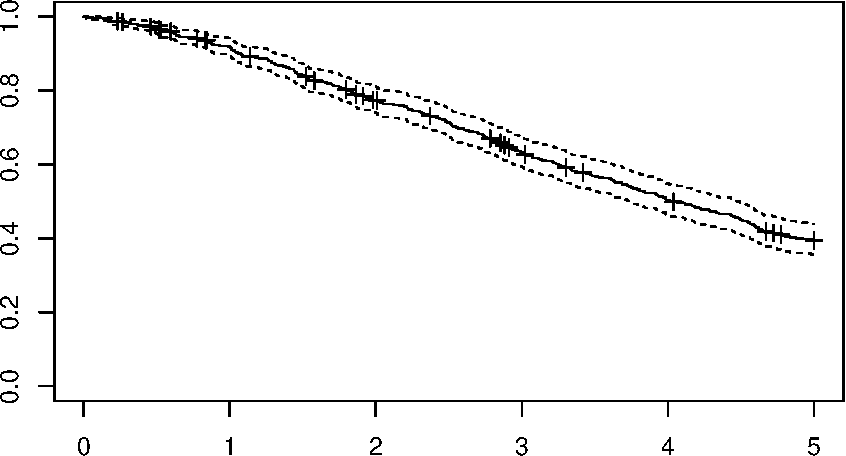
\includegraphics[width=1\linewidth]{decision_tree_HVE_solutions_files/figure-latex/unnamed-chunk-6-1}

\hypertarget{cost-effectiveness-analysis}{%
\subsection{05 Cost-Effectiveness
Analysis}\label{cost-effectiveness-analysis}}

\begin{Shaded}
\begin{Highlighting}[]
\CommentTok{# create the transition probability matrix for NO treatment}
\NormalTok{decision_tree_HVE_cea  <-}\StringTok{ }\KeywordTok{calculate_icers}\NormalTok{(}\DataTypeTok{cost       =}\NormalTok{ decision_tree_HVE_output}\OperatorTok{$}\NormalTok{Cost,}
                                          \DataTypeTok{effect     =}\NormalTok{ decision_tree_HVE_output}\OperatorTok{$}\NormalTok{Effect,}
                                          \DataTypeTok{strategies =}\NormalTok{ decision_tree_HVE_output}\OperatorTok{$}\NormalTok{Strategy)}
\NormalTok{decision_tree_HVE_cea}
\end{Highlighting}
\end{Shaded}

\begin{verbatim}
##   Strategy     Cost   Effect Inc_Cost Inc_Effect     ICER Status
## 1    No Tx  4117.20 19.62600       NA         NA       NA     ND
## 2   Tx All 12908.96 19.71680  8791.76     0.0908 96825.55     ND
## 3   Biopsy 32599.41 19.69896       NA         NA       NA      D
\end{verbatim}

\hypertarget{plot-frontier-of-decision-tree}{%
\subsection{05.1 Plot frontier of Decision
Tree}\label{plot-frontier-of-decision-tree}}

\begin{Shaded}
\begin{Highlighting}[]
\KeywordTok{plot}\NormalTok{(decision_tree_HVE_cea, }\DataTypeTok{effect_units =} \StringTok{"QALYs"}\NormalTok{, }\DataTypeTok{label=}\StringTok{"all"}\NormalTok{)}
\end{Highlighting}
\end{Shaded}

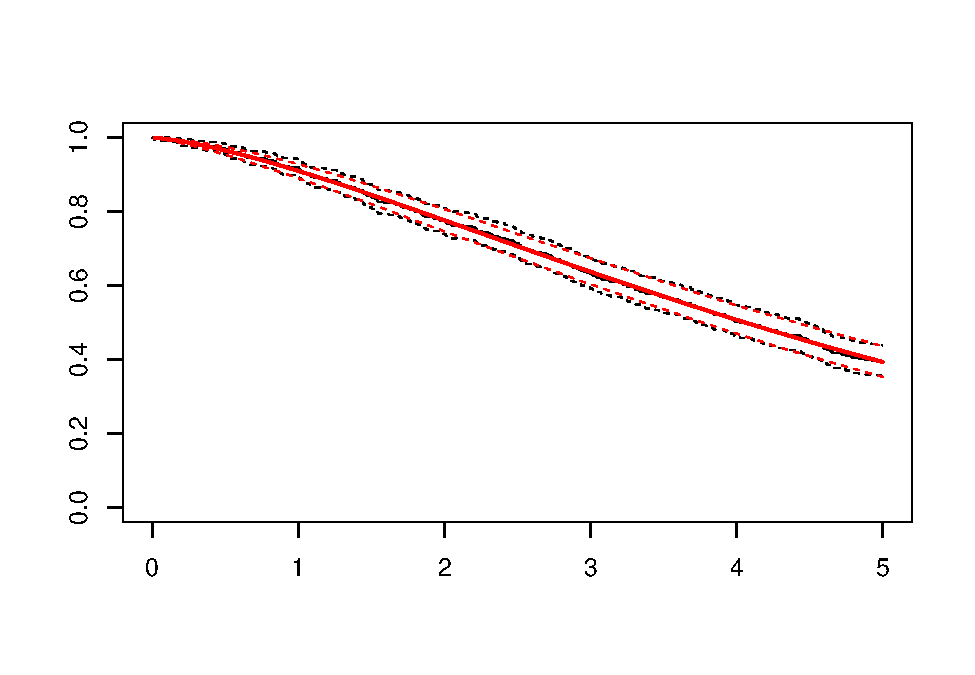
\includegraphics{decision_tree_HVE_solutions_files/figure-latex/unnamed-chunk-8-1.pdf}

\end{document}
